\label{setup}
In order to gain a deeper understanding of the performance dynamics outlined in ~\S\ref{subsec:model} and ~\S\ref{subsec:model_fitting}, we need to experimentally evaluate questions about how caching affects PLT in a controlled environment.
%Our goal for the rest of the paper is to gain a deeper understanding of the performance dynamics outlined in the previous section.
%To do so  we need to experimentally evaluate, in a controlled manner, questions about how caching affects performance.
Here, we develop our methodology.
% To achieve our goal, we must address the following challenge:

Our experimental apparatus (publicly available at~\cite{jamshed-telemetry}) makes use of Telemetry~\cite{telemetry} and Web Page Replay (WPR)~\cite{wpr} to measure the effects of parameterized levels of network delays.
Both Telemetry and WPR are part of Chromium~\cite{chromium-source}, the open source components of Google Chrome.
Here, we use the term `browser' interchangeably with Google Chrome.

\textbf{Web Page Replay}. WPR acts as a local DNS and HTTP(S) proxy cache (depicted in Figure~\ref{fig:workflow_diagram}a).
In record mode, WPR forwards HTTP(S) requests to the Internet, and records all requests and responses that it observes, as well as metadata such as observed network delays. From this, Web Page Replay builds a WPR archive (depicted in Figure~\ref{fig:workflow_diagram}b), complete with all HTTP(S) requests, responses, headers, data, and network delays. % the last part of this sentence is somewhat redundant.

In replay mode, the WPR proxy responds to HTTP(S) requests with the responses saved in the archive, or a 404 error response if the corresponding response is not saved in the archive.
We configure WPR to send the matching response and data only after sleeping for the time duration originally observed as the network delay between the origin and the WPR proxy (while it was in record mode). Here, WPR is emulating an edge cache rather than a browser cache.

\textbf{Telemetry}. Telemetry (Figure~\ref{fig:workflow_diagram}c) is a browser performance testing framework, which orchestrates the behavior of the browser and WPR.
We use Telemetry to control one of two browsers. The first is a desktop version of Google Chrome running within a virtual machine (specifications in ~\ref{specs}). The second is a mobile version of Google Chrome running on a USB-tethered mobile device.
We use Telemetry to load requested URLs in the browser (as if the user is entering URLs into the omnibox) and passively measuring PLT.
\subsection{Workflow} \label{workflow}
\begin{figure}[t]
    \hspace{-10pt}
    \figuretitle{Experimental Apparatus Workflow}
    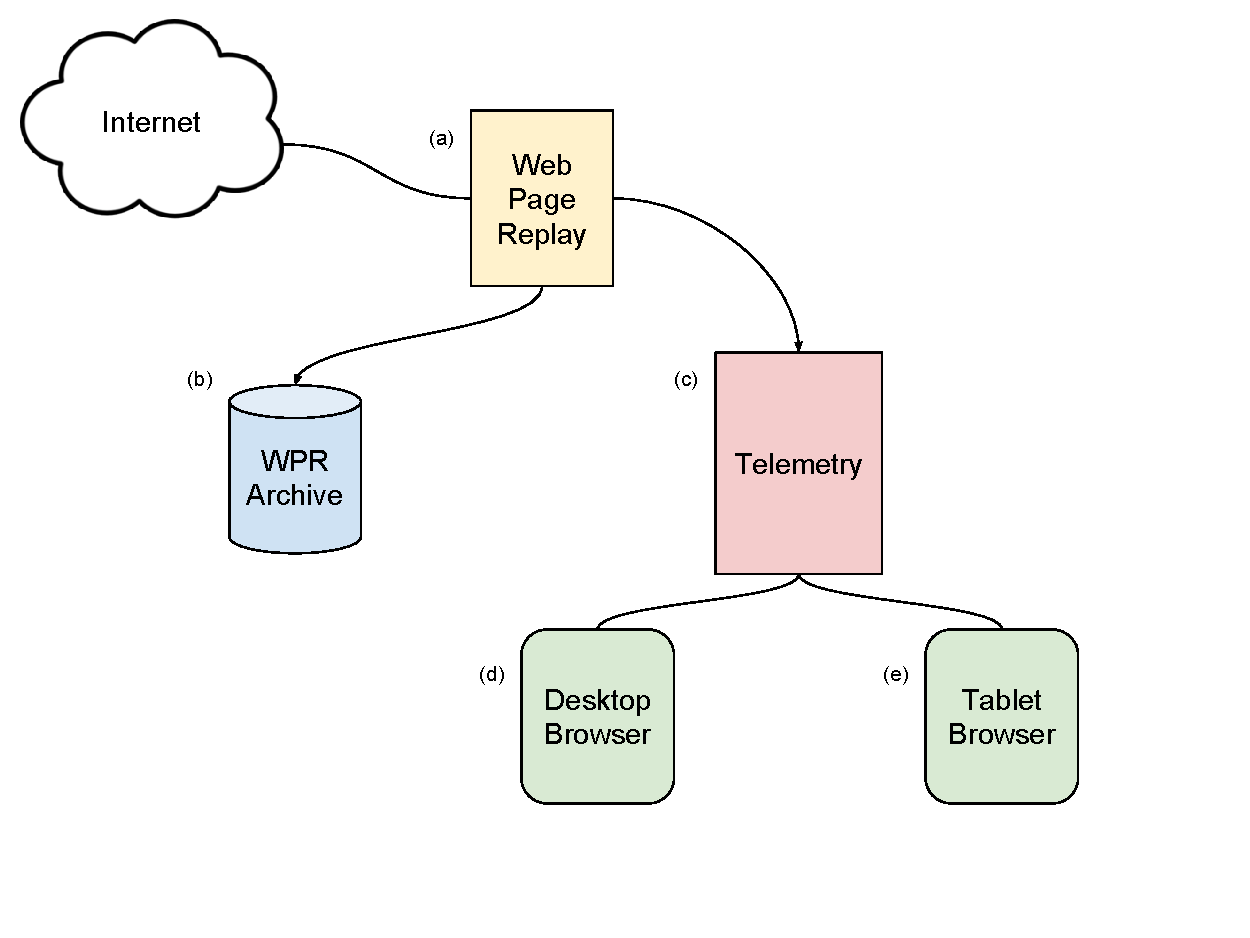
\includegraphics[width=3in]{../images/methodology_workflow_diagram.pdf}
    \caption[]{\label{fig:workflow_diagram}Logical units of our apparatus.}
\end{figure}

\begin{figure*}[!htb]
\hspace{0.01in}
\begin{subfigure}{0.33\textwidth}
    \hspace*{-0.11in}
    \figuretitle{Cacheable Bytes} 
    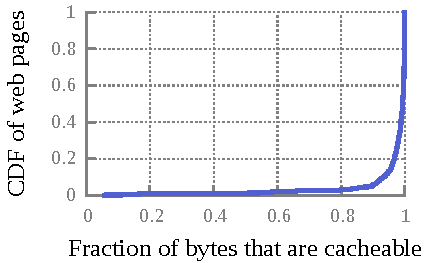
\includegraphics[width=\textwidth]{../graphs/cacheable_bytes/cacheable_bytes_linear.pdf}
    \caption[]{\label{fig:cacheable_bytes_linear}}
\end{subfigure}\hfill
\begin{subfigure}{0.33\textwidth}
    \hspace*{-0.11in}
    \figuretitle{Total Bytes} 
    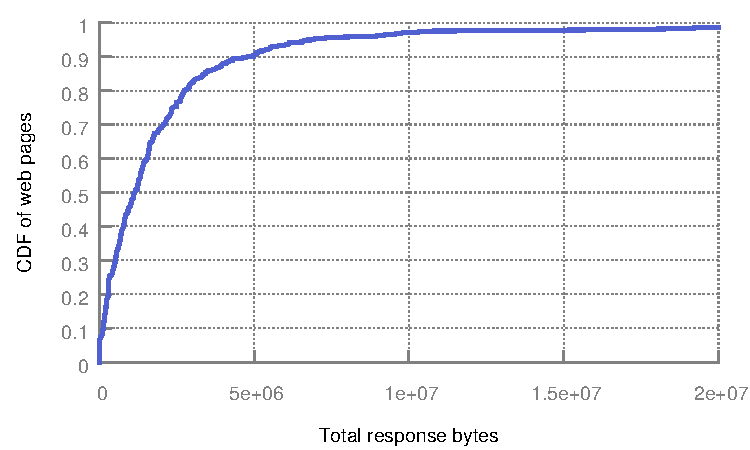
\includegraphics[width=\textwidth]{../graphs/total_bytes/total_bytes_linear.pdf}
    \caption[]{\label{fig:total_bytes_linear}}
\end{subfigure}\hfill
\begin{subfigure}{0.33\textwidth}
    \hspace*{-0.11in}
    \figuretitle{Partial Cache Page Load Time} 
    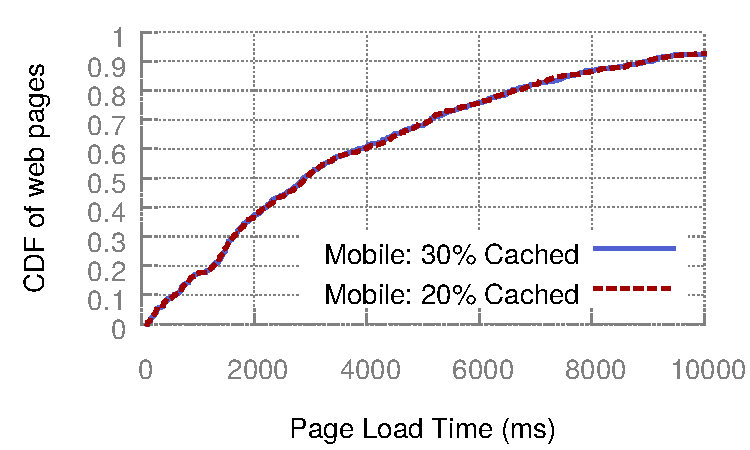
\includegraphics[width=\textwidth]{../graphs/partial_cache/partial_cache_linear_PLT.pdf}
    \caption[]{\label{fig:partial_cache_linear}}
\end{subfigure}\hfill
\caption{(\ref{fig:cacheable_bytes_linear}): The majority of web pages are composed mostly of cacheable bytes. (\ref{fig:total_bytes_linear}): While 95\% of web pages are under 6.8 MB, the median web page size is less than 1.2 MB. (\ref{fig:partial_cache_linear}): Increasing the cache hit ratio from 20\% to 30\% had negligible effects on mobile PLT.}
\end{figure*}
Before each experiment, we clear the browser cache to ensure consistency across trials. For each device (desktop and mobile), we execute the following steps for each URL:

%\colin{If we're looking to cut space, we might make this more terse, since it's redundant with above}
First, we record the live web page from the Internet using Telemetry to instruct the browser to fetch the given URL. The WPR proxy receives this HTTP(S) request, forwards it to the Internet, and passively inspects and records the two-way traffic as noted in (\ref{setup}). This data is stored as a WPR archive.

Next, we determine the page load time of the web page with a cold cache. With WPR in replay mode, we load the URL four times (see~\ref{known_limitations}) and take the minimum page load time as our PLT value, to account for variance.

Now, we emulate a ``perfect,'' fully populated cache. First, we copy the original WPR archive into a new WPR archive. For each cacheable response in this new WPR archive, we set its network delay to 0 (of course, a ``real" cache response time of 0 is not possible, but we set this as an absolute lower bound). Non-cacheable items, as indicated by HTTP headers, retain their initial network delays. We store this modified archive alongside the original (Figure~\ref{fig:workflow_diagram}b).

Lastly, we record the page load time again, however this time using the modified WPR archive. We determine the PLT in the same way as the original. We then compare the page load times of the unmodified replay executions to that of the modified ``perfect cache'' executions.

\textbf{Partial Caching}. To confirm Flywheel's findings, we created two additional sets of partially cached WPR archives: one that caches a uniformly randomly chosen set of 30\% of all cacheable resources (regardless of byte size), and another that caches 20\%.
We ensure that the cached items in the 20\% WPR archive are a strict subset of the cached items in the 30\% WPR archive for consistency. 
%\arvind{this is the bit which might need justification; why is random the right choice? let us say that I visit cnn.com.  Shouldn't all of the resources inside cnn.com - say js, css, etc. - be either cached or not cached?  Does it make sense for js to be cached and not css?}
%\jamshed{Whole Objects, not bytes, and taking a uniform random distribution}
\subsection{Specifications} \label{specs}
Each web page was originally fetched over UC Berkeley's LAN, which approximates 250 Mbps down and 230 Mbps up.
Our mobile device is a Galaxy Tab 4 with a 1.2 GHz quad-core processor and 1.5 GB on board RAM running Android 4.4, KitKat. Desktop results were performed in a virtual machine with a 3.2 GHz quad-core processor and 6 GB RAM.
%\arvind{maybe this should be pitched as an edge cache?  maybe the fact that this is an edge cache makes the random choice above more palatable?}
\subsection{Known Limitations}  \label{known_limitations}
We identify the following apparatus limitations and discuss the reasoning behind our choice of tools:

%\colin{We can cut this if we need space. Don't really need to defend this choice.}
\textbf{Page Load Time as a Metric}. When determining web page performance, we chose to focus on page load time rather than SpeedIndex~\cite{speed-index} or above-the-fold time~\cite{above-the-fold}.
Although they are arguably preferable metrics (as they do a better job of capturing the user's perspective), these metrics are significantly more difficult to measure consistently.
%Further, other metrics do not necessarily account for below-the-fold Javascript or other background resources that may cause significant delays to a user's final experience of a web page.

\textbf{WPR Measurement Accuracy}. The PLT measurements taken by WPR are not necessarily consistent with PLTs observed on live web pages, nor are they necessarily consistent across multiple runs of WPR. First, although WPR attempts to mitigate non-determinism in JavaScript execution (by injecting a script into each webpage that interposes on non-deterministic calls such as \texttt{getTime}), JavaScript may nonetheless exhibit non-determinism across different loads. Second, the mechanism WPR uses to emulate the original RTTs observed during record mode  (sleeping a fixed number of milliseconds) may not perfectly match the behavior of the original page load.
%These artifacts affect both mobile and desktop browsers in the same manner.
We try to mitigate these artifacts by loading each web page four times and
taking the minimum PLT.\footnote{We observed that beyond four loads per web
page, the minimum PLT value did not decrease significantly.}
%\textbf{WPR Interference}. In our apparatus, the WPR proxy acts as a middlebox between the client and the web content. While we make this proxy transparent, it is possible that it interferes with our experiment. \jamshed{add or remove}.
